\documentclass[]{tufte-handout}

% ams
\usepackage{amssymb,amsmath}

\usepackage{ifxetex,ifluatex}
\usepackage{fixltx2e} % provides \textsubscript
\ifnum 0\ifxetex 1\fi\ifluatex 1\fi=0 % if pdftex
  \usepackage[T1]{fontenc}
  \usepackage[utf8]{inputenc}
\else % if luatex or xelatex
  \makeatletter
  \@ifpackageloaded{fontspec}{}{\usepackage{fontspec}}
  \makeatother
  \defaultfontfeatures{Ligatures=TeX,Scale=MatchLowercase}
  \makeatletter
  \@ifpackageloaded{soul}{
     \renewcommand\allcapsspacing[1]{{\addfontfeature{LetterSpace=15}#1}}
     \renewcommand\smallcapsspacing[1]{{\addfontfeature{LetterSpace=10}#1}}
   }{}
  \makeatother

\fi

% graphix
\usepackage{graphicx}
\setkeys{Gin}{width=\linewidth,totalheight=\textheight,keepaspectratio}

% booktabs
\usepackage{booktabs}

% url
\usepackage{url}

% hyperref
\usepackage{hyperref}

% units.
\usepackage{units}


\setcounter{secnumdepth}{2}

% citations

% pandoc syntax highlighting

% longtable
\usepackage{longtable,booktabs}

% multiplecol
\usepackage{multicol}

% strikeout
\usepackage[normalem]{ulem}

% morefloats
\usepackage{morefloats}


% tightlist macro required by pandoc >= 1.14
\providecommand{\tightlist}{%
  \setlength{\itemsep}{0pt}\setlength{\parskip}{0pt}}

% title / author / date
\title{TP2 - Reconocimiento de Patrones}
\author{Elio Campitelli}
\date{}

\usepackage{booktabs}
\usepackage{longtable}
\usepackage{array}
\usepackage{multirow}
\usepackage{wrapfig}
\usepackage{float}
\usepackage{colortbl}
\usepackage{pdflscape}
\usepackage{tabu}
\usepackage{threeparttable}
\usepackage{threeparttablex}
\usepackage[normalem]{ulem}
\usepackage{makecell}
\usepackage{xcolor}

\begin{document}

\maketitle



{
\setcounter{tocdepth}{2}
\tableofcontents
}

\hypertarget{datos}{%
\section{Datos}\label{datos}}

En este TP voy a estar usando la base de datos \texttt{penguins} del paquete de R \textbf{palmerpenguins} (KB, TD, and WR 2014). Los datos recolectados por la Dra. Kristen Gorman en la Estación Palmer, consisten en mediciones de la longitud del culmen\footnote{El culmen es la parte superior del pico de las aves 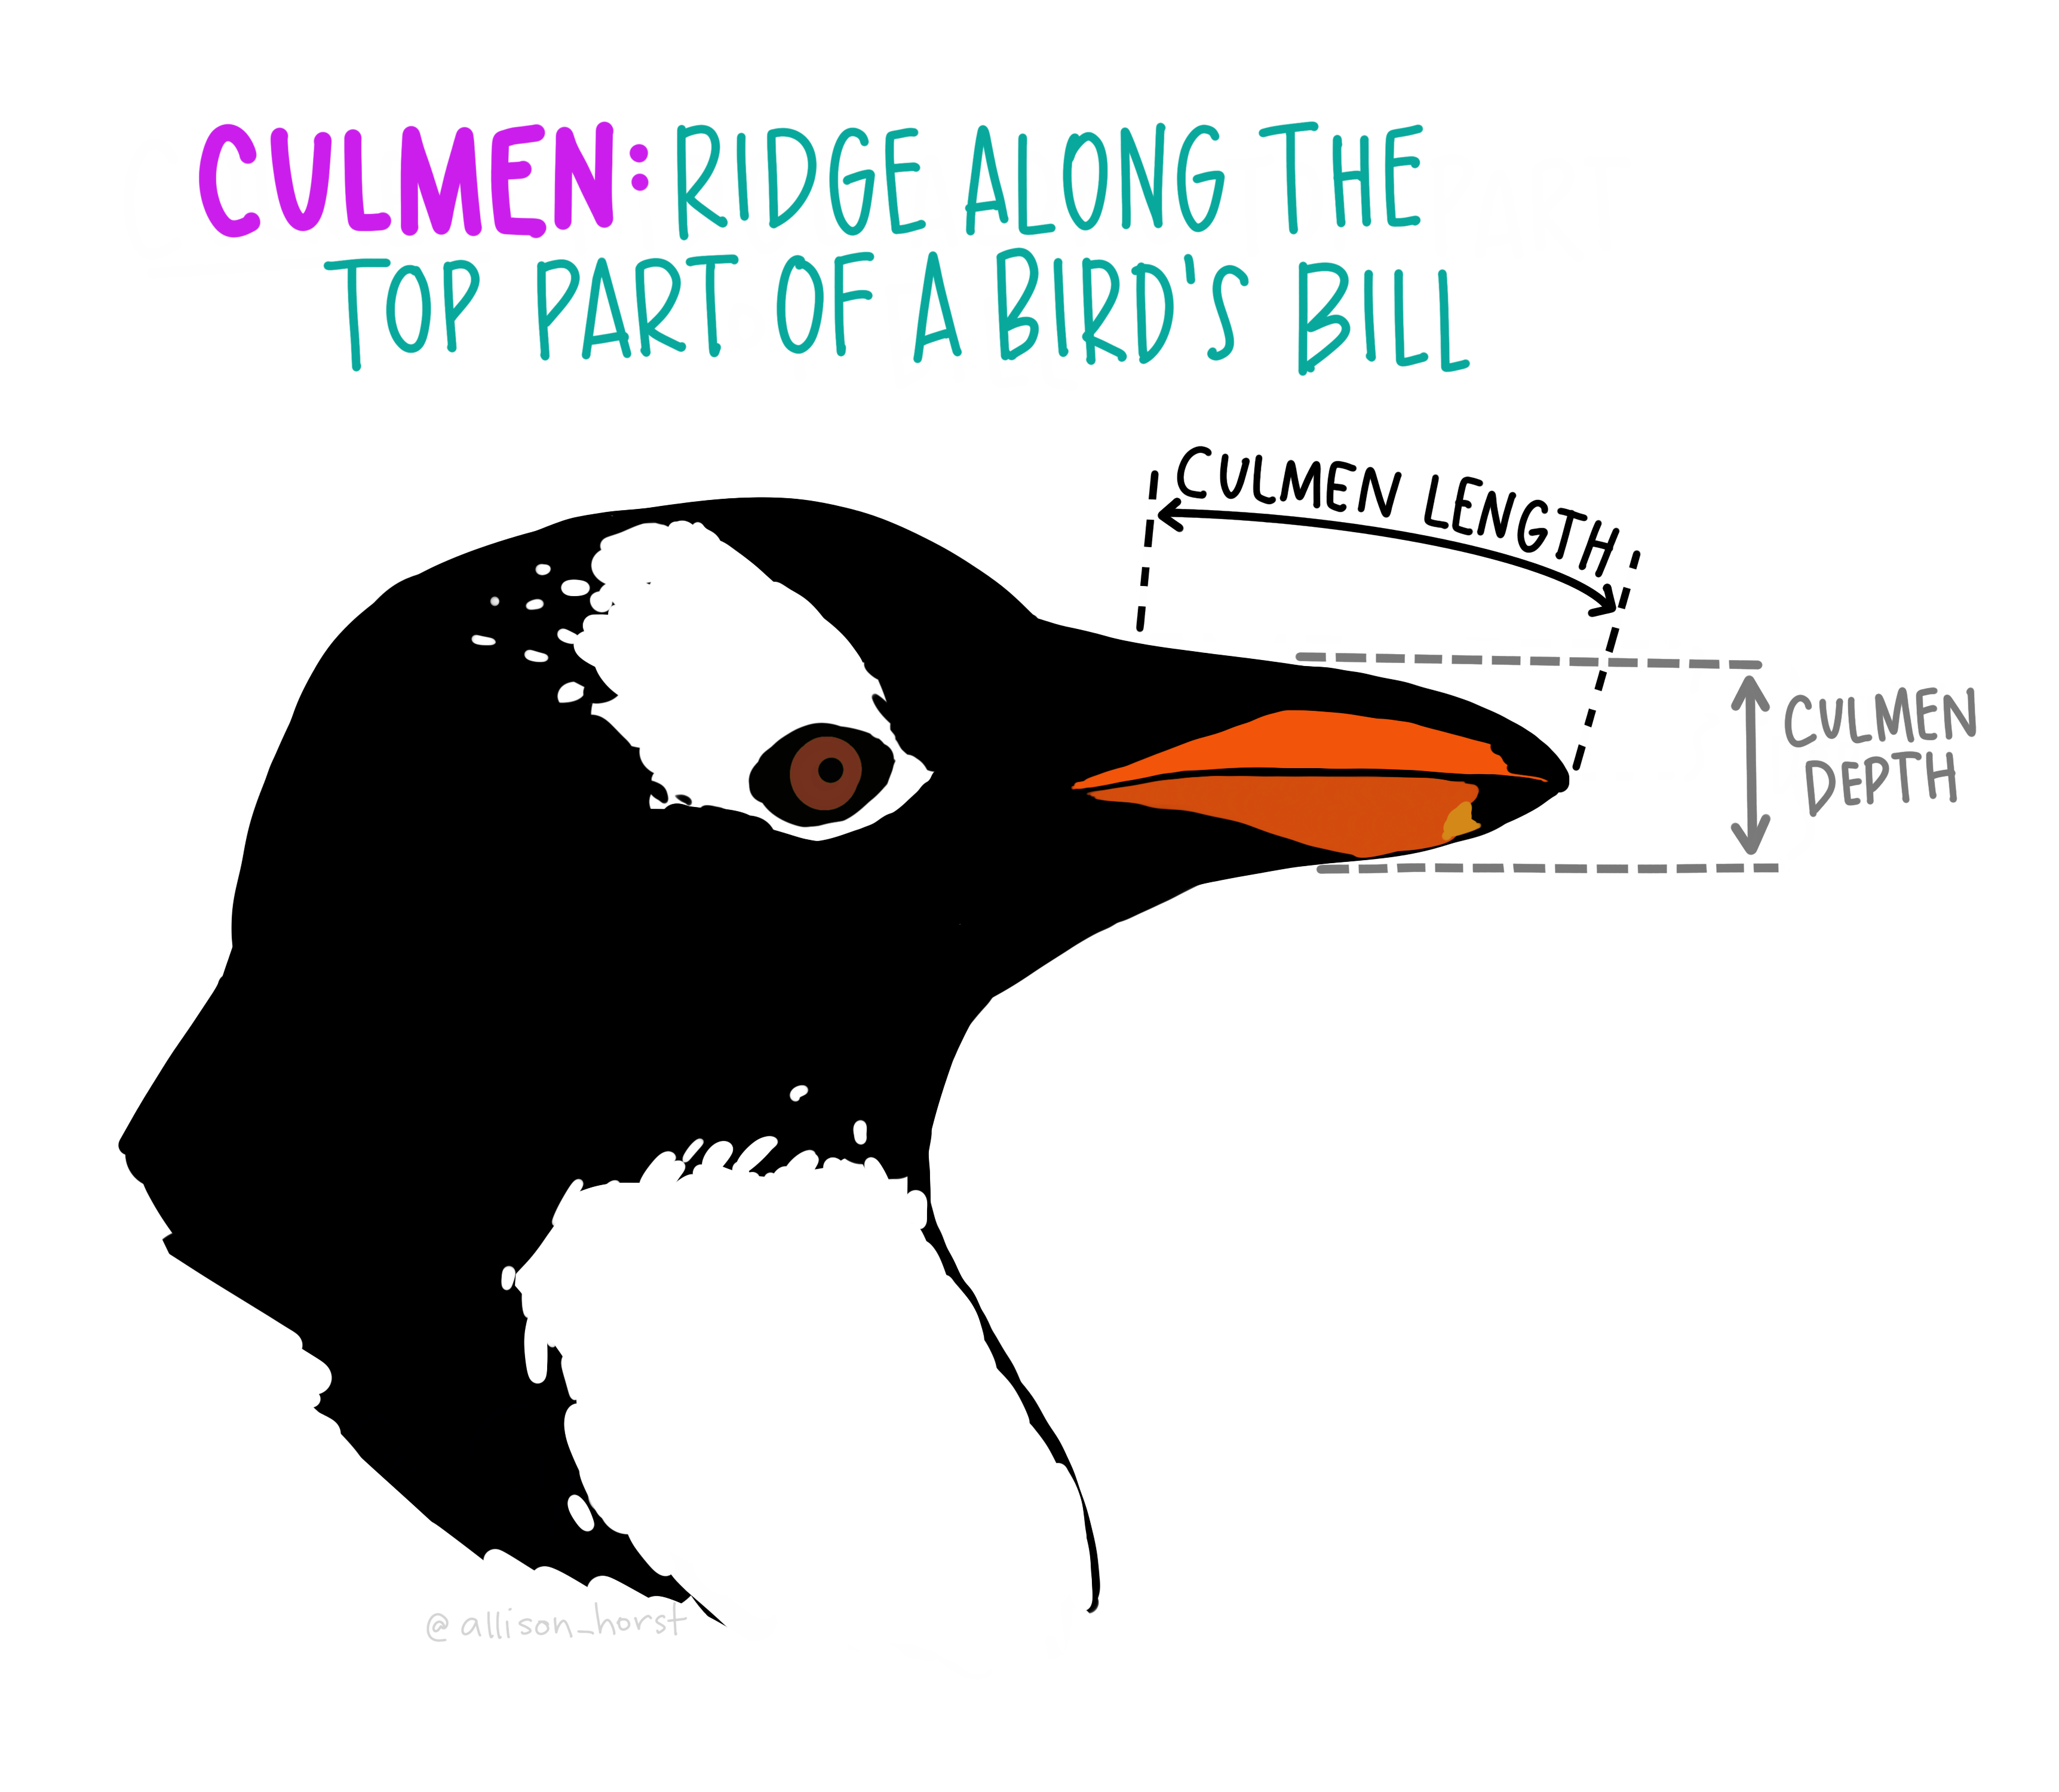
\includegraphics{culmen_depth.png}}, alto del culmen y la masa corporal de 342 pingüinos de las especies \emph{Pygoscelis adeliae} (Pingüino de Adelaida), \emph{Pygoscelis papua} (Pingüino Juanito), y \emph{Pygoscelis antarcticus} (Pingüino barbijo).

\begin{center}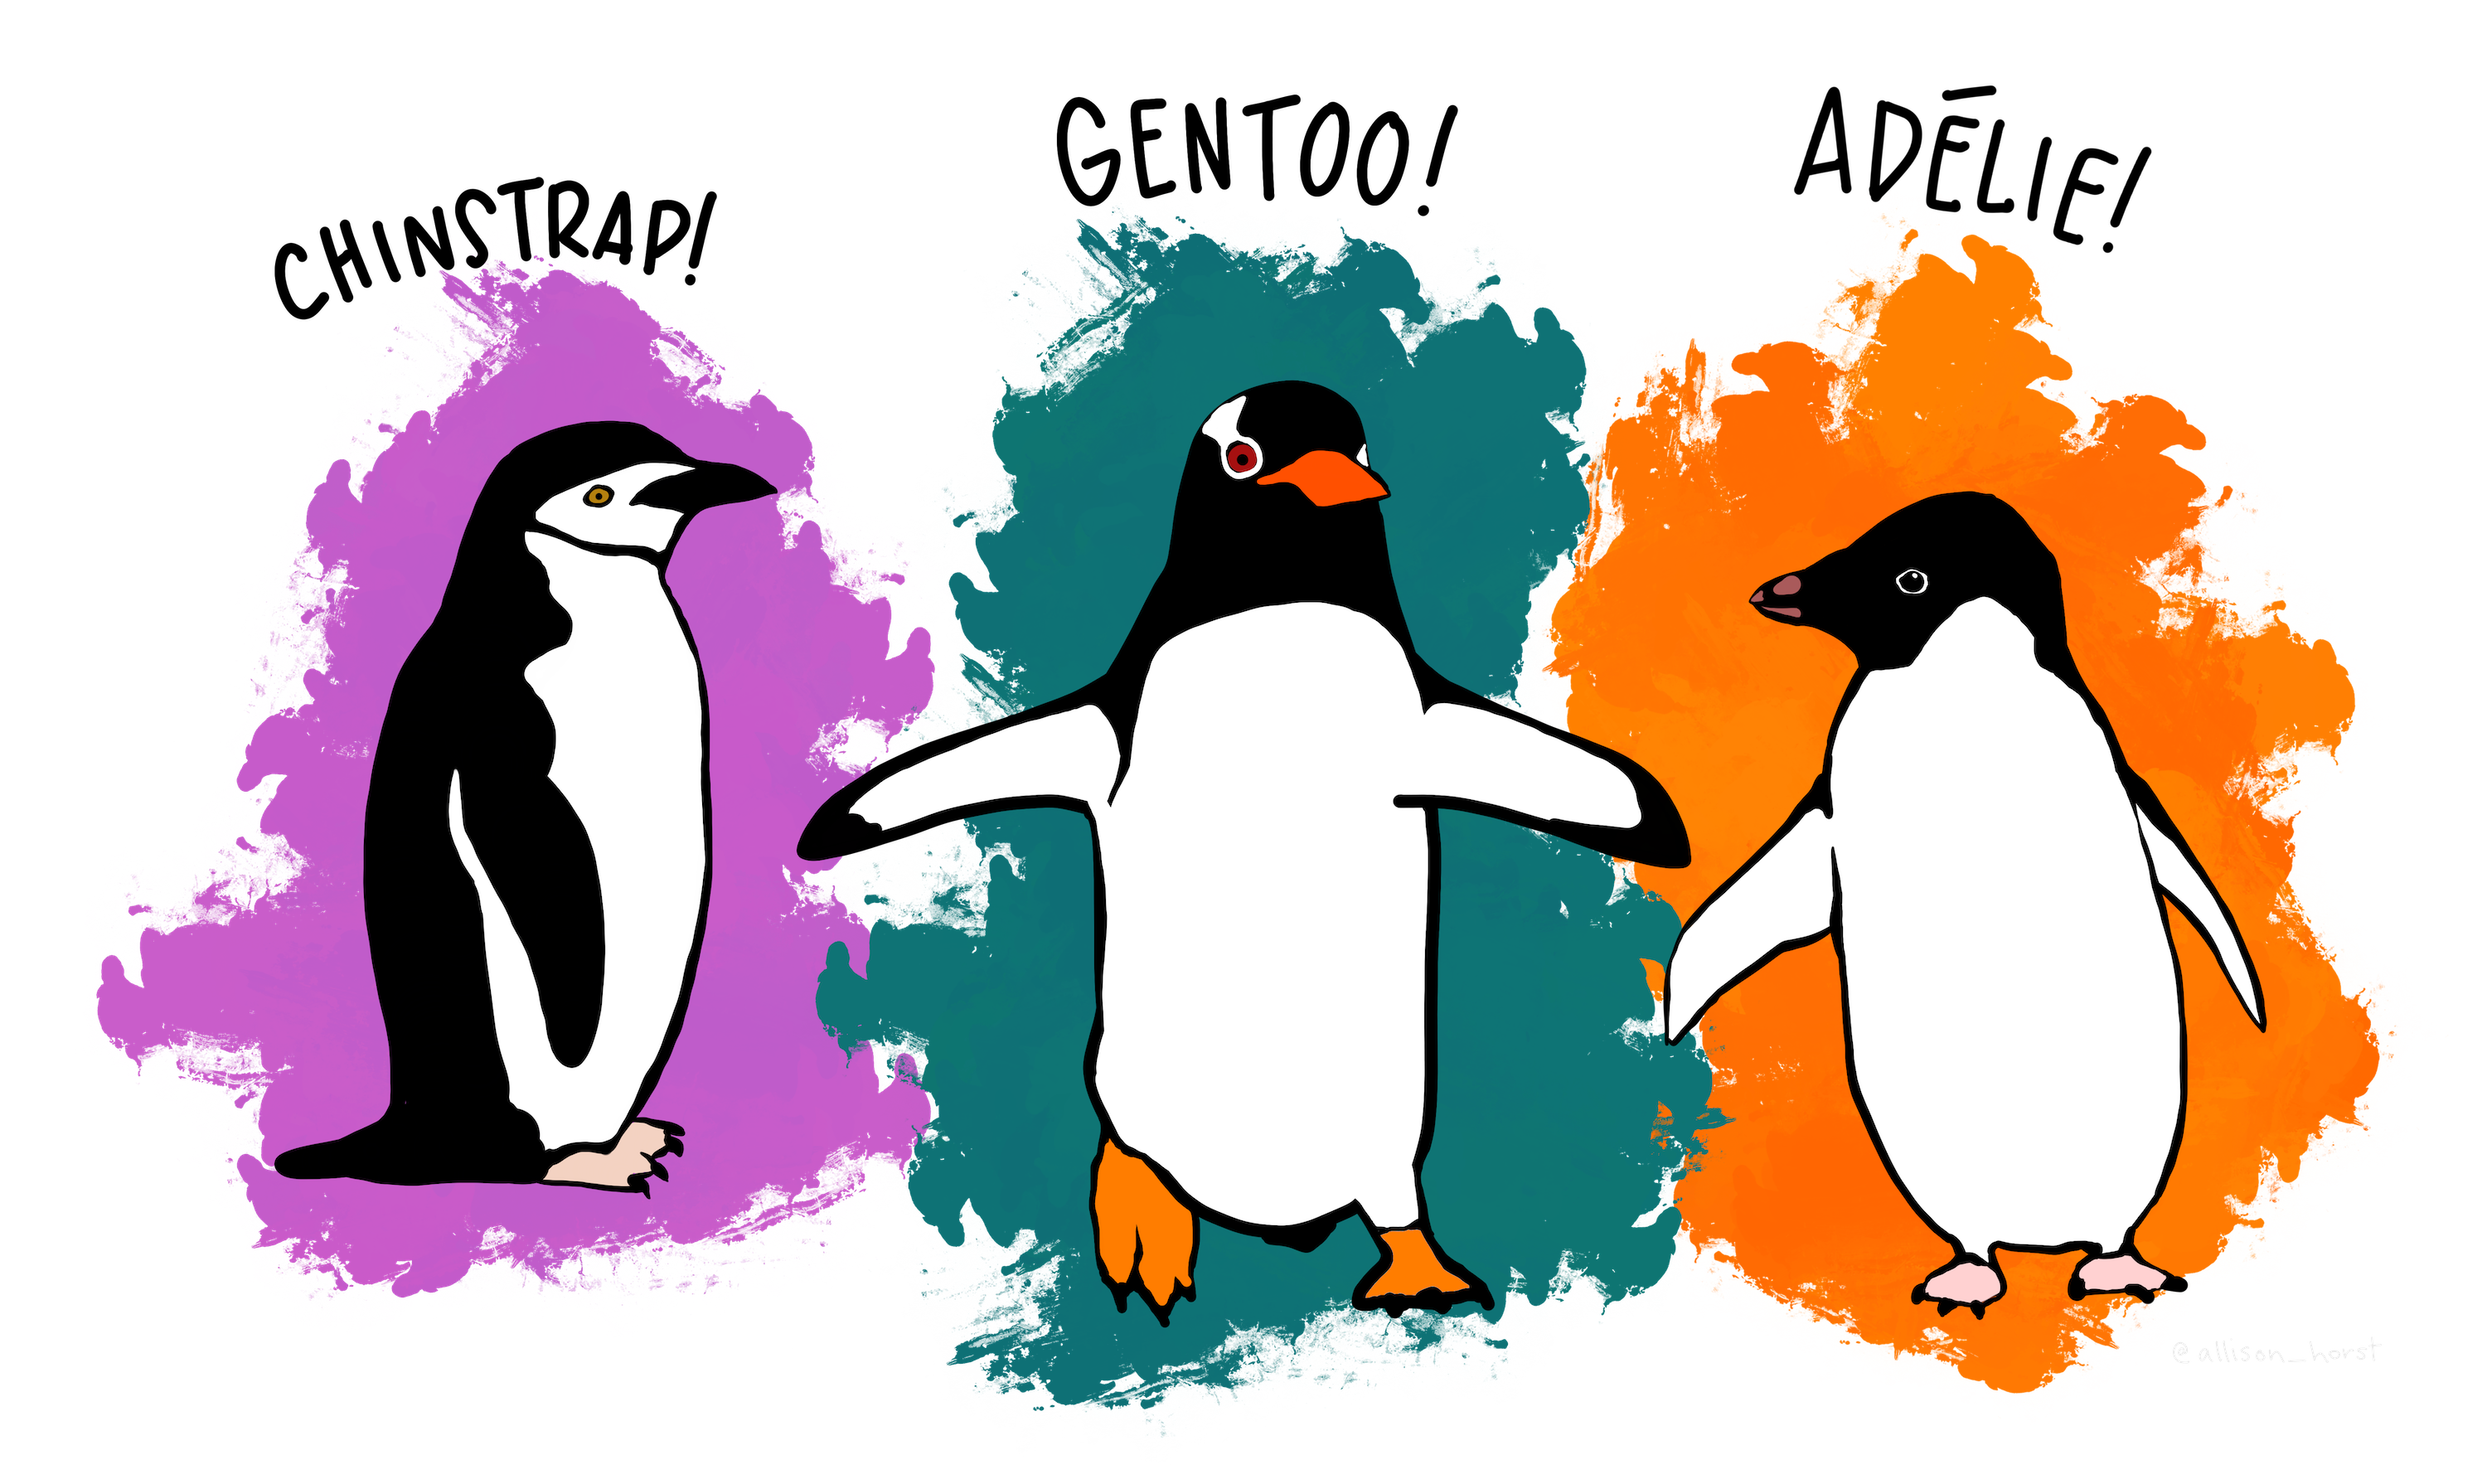
\includegraphics[width=0.8\linewidth]{penguins} \end{center}

En la Tabla \ref{tab:pen-glance} se muestran las primeras 3 mediciones para cada especie.

\begin{table}

\caption{\label{tab:pen-glance}Primeras 3 entradas de cada especie en los datos utilizados}
\centering
\begin{tabular}[t]{l>{\raggedleft\arraybackslash}p{2cm}>{\raggedleft\arraybackslash}p{2cm}>{\raggedleft\arraybackslash}p{2cm}>{\raggedleft\arraybackslash}p{2cm}}
\toprule
Especie & Longitud de culmen [mm] & Alto de culmen [mm] & Longitud de la aleta [mm] & Masa corporal [g]\\
\midrule
adelaida & 39.1 & 18.7 & 181 & 3750\\
adelaida & 39.5 & 17.4 & 186 & 3800\\
adelaida & 40.3 & 18.0 & 195 & 3250\\
juanito & 46.1 & 13.2 & 211 & 4500\\
juanito & 50.0 & 16.3 & 230 & 5700\\
\addlinespace
juanito & 48.7 & 14.1 & 210 & 4450\\
barbijo & 46.5 & 17.9 & 192 & 3500\\
barbijo & 50.0 & 19.5 & 196 & 3900\\
barbijo & 51.3 & 19.2 & 193 & 3650\\
\bottomrule
\end{tabular}
\end{table}

La variable categórica a predecir va a ser la especie, y las posibles variables predictoras son las dimensiones del culmen, la longitud de la aleta y la masa corporal. Es decir, en principio es un espacio de dimensión 4. Como la idea es trabajar en \(\mathbb{R}^2\), conviene explorar qué grado de separación permite cada combinación de dos variables. Esto se muestra en la Figura \ref{fig:pairs} donde se grafican scatterplots para todas las combinaciones de dos variables con la especie representada con color. Mirando las densidades de probabilidad (gráficos en la diagonal) se puede ver que la longitud del culmen separa bastante bien entre pingüino de adelaida y el resto mientras que las otras variables separan bien al pingüino juanito. Por lo tanto, las combinaciones que incluyen la longitud del culmen (gráficos en la primera columna) separan bastante bien entre las tres especies, mientras que el resto de las combinaciones tienen algún grado de mezcla entre pingüino de adelaida y pingüino juanito.

\begin{figure*}
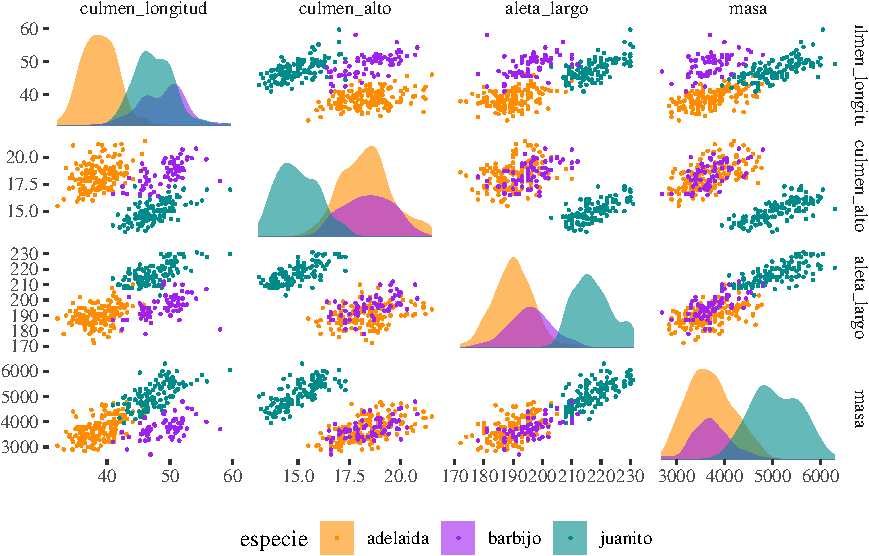
\includegraphics{TP-Labo-2_files/figure-latex/pairs-1} \caption[Scatteplot de todas las combinaciones de variables posibles en $\mathbb{R}^2$]{Scatteplot de todas las combinaciones de variables posibles en $\mathbb{R}^2$. En la diagonal, estimaciones de densidad de cada variable separadas por especies.}\label{fig:pairs}
\end{figure*}

Para hacer las cosas más interesantes, voy a seleccionar el espacio formdado por el largo de la aleta y la masa. En este espacio \(\mathbb{R}^2\), los piingüinos juanitos se separan muy bien de los otros, pero los adelaida y los barbijo están mezclados y son imposibles de separar.

\begin{figure*}
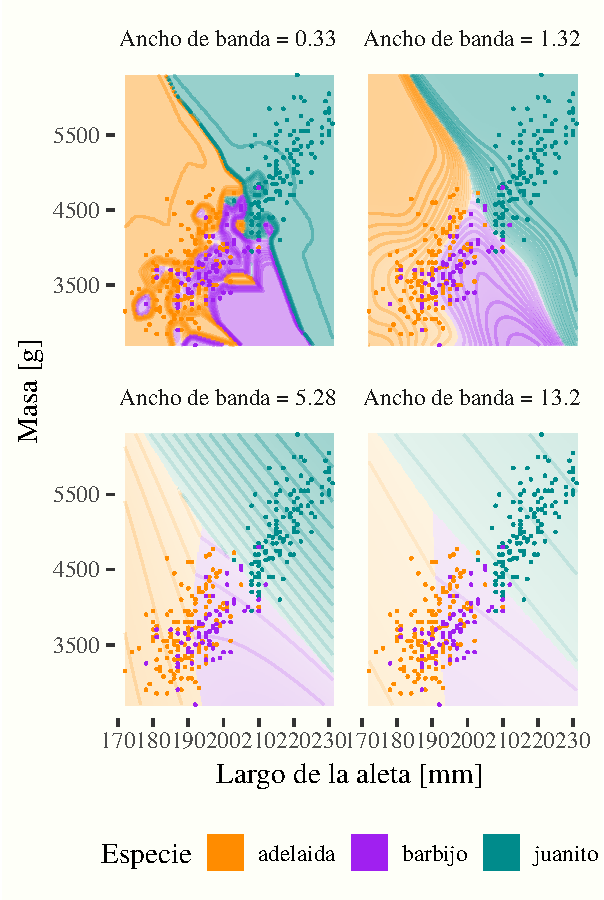
\includegraphics{TP-Labo-2_files/figure-latex/densidad-1} \caption[Separación del espacio a partir de estimar la densidad con un kernel gausiano de distintos anchos de banda]{Separación del espacio a partir de estimar la densidad con un kernel gausiano de distintos anchos de banda.}\label{fig:densidad}
\end{figure*}

La Figura \ref{fig:densidad} muestra distintas particiones posibles del espacio a partir de estimar las densidades de probabilidad conjunta de cada clase y asignando la clase con mayor densidad de probabilidad en cada punto\footnote{Dada la diferencia de escalas de x e y, en principio el valor del ancho de banda no podría ser el mismo para ambas dimensiones. Para armonizarlas, se hicieron los cálculos en base a las variables estandarizadas}. Cuando el ancho de banda es muy pequeño, se observa que el clasificación sufre de overfitting. Las regiones clasifican perfectamente los datos observados, pero los límites de decisión se curva para rodear puntos aislados. Para un ancho de banda muy grande, los límites de decisión tidneden a rectas y se ve que las estimaciones de densidad son círculos concéntricos que ignoran la covarianza entre los datos.

\hypertarget{clasificador-cuadruxe1tico}{%
\section{Clasificador cuadrático}\label{clasificador-cuadruxe1tico}}

La función \texttt{clasificador\_cuadratico} genera un modelo lineal de clasificación que es esencialmente un modelo lineal multivariado donde las \(K\) variables dependientes representan a las \(K\) categorías usando one-hot encoding. Es decir, el modelo tiene \(M\) predictores y \(K\) predicciones, una para cada clase. La clasificación se hace asignando la clase que tiene el valor máximo. Como medida de la confianza del resultado, se toma la razón entre ese valor máximo y la suma de todos los valores asignados a cada clase)

La partición del espacio \(\mathbb{R}^2\) elegido usando el resultado del clasificador cuadrático se muestra en la Figura \ref{fig:cuadratico}. Dado que el clasificador es lineal, las divisiones entre categorías son rectas que se interceptan en un punto central.

\begin{figure}
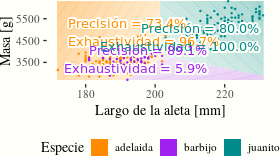
\includegraphics{TP-Labo-2_files/figure-latex/cuadratico-1} \caption[Clasificación en base a clasificador cuadrático lineal]{Clasificación en base a clasificador cuadrático lineal. En contornos negros, el nivel de confianza del modelo. "Precisión" se define como la proporción de observaciones clasificadas como una determinada especie que fueron clasificadas correctamente, "Exhaustividad" se define como la proporción de observaciones de cada especie correctamente clasificadas.}\label{fig:cuadratico}
\end{figure}

Se muestran dos medidas de la clasificación para cada especie. ``Exhaustividad'' es la proporción de observaciones que son clasificadas como una especie de forma correcta. ``Precisión'' es la proporción de observaciones de una determinada especie que son clasificadas correctamente. Es decir, la exhaustividad del 100\% para los pingüinos juanitos implica que la probabilidad de que un pingüino juanito sea correctamente clasificado es del 100\%. Sin embargo, la precisión del 80\% implica que si el modelo clasifica un pingüino como juanito, hay un 80\% de probabilidad de que haya sido clasificado correctamente.
Se puede ver que si bien el clasificador lineal cuadrático identifica sin problemas a los pingüinos juanito, la separación entre adelaida y barbijo no es para nada buena.

\hypertarget{loguxedstica}{%
\subsection{Logística}\label{loguxedstica}}

La función \texttt{logistica} realiza el ajuste logístico mediante un método iterativo. Soporta clasificación de múltiples clases usando el algoritmo de uno-vs-todos. Es decir, para \(K\) clases genera \(K\) modelos que dan la probabilidad de que una observación determinada pertenezca a la clase k-ésima o a cualquiera de las otras. La clasificación luego se hace tomando la clase que tiene la mayor probabilidad. Al igual que con el clasificador cuadrático, como medida de confianza del modelo se calcula la razón entre la probabilidad asignada a la clase ganadora y la suma de todas las probabilidades asignadas.

\begin{figure}
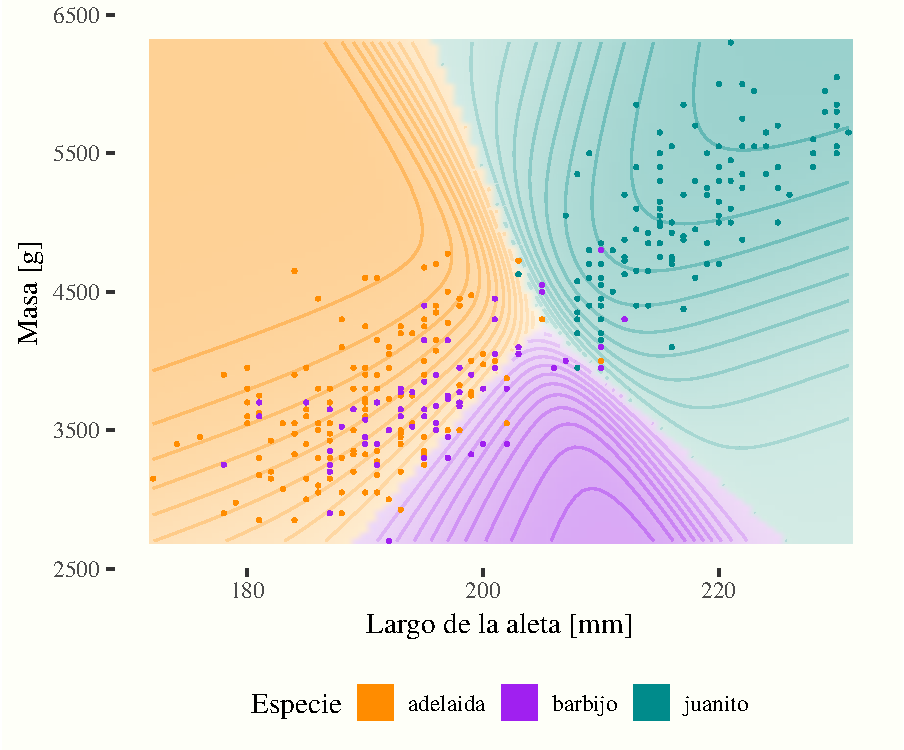
\includegraphics{TP-Labo-2_files/figure-latex/logistica-lineal-1} \caption[Convergencia del modelo logístico lineal]{Convergencia del modelo logístico lineal. En contornos negros, el nivel de confianza del modelo.}\label{fig:logistica-lineal}
\end{figure}

La Figura \ref{fig:logistica-lineal} muestra el resultado de la clasificación logística lineal. Al igual que con la Figura \ref{fig:cuadratico}, los límites de decisión son rectas dado qu eel modelo es linear en este espacio \(\mathbb{R}^2\). La partición no es muy distinta de la partición usando el clasificador cuadrático. La Figura \ref{fig:logistica-eliptica}, en cambio, muestra el resultado del modelo logístico pero aplicado al espacio de dimensión 4 \((x, y, x^2, y^2, xy)\). Al tener términos no lineales, los límites de decisión ahora pueden ser curvos\footnote{Son curvos en el espacio \(\mathbb{R}^2\) mostrado, en el espacio de dimensión 4, siguen siendo rectas.}

\begin{figure}
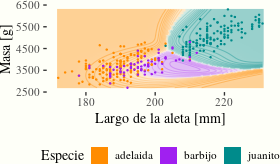
\includegraphics{TP-Labo-2_files/figure-latex/logistica-eliptica-1} \caption[Igual que la Figura \\ref{fig:logistica-lineal} pero para un ajuste elíptico]{Igual que la Figura \\ref{fig:logistica-lineal} pero para un ajuste elíptico.}\label{fig:logistica-eliptica}
\end{figure}

\hypertarget{expectation-maximisation}{%
\section{Expectation Maximisation}\label{expectation-maximisation}}

Expectation maximisation (EM) es una técnica no supervisada, es decir, que no tiene en cuenta las clases observadads.

\begin{figure}
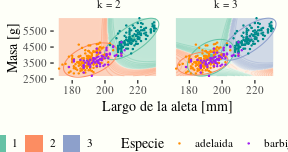
\includegraphics{TP-Labo-2_files/figure-latex/em-pinguinos-1} \caption[Media y elipse normal ]{Media y elipse normal }\label{fig:em-pinguinos}
\end{figure}

La Figura \ref{fig:em-pinguinos} muestra el resultado del algoritmo de EM con los datos de pingüinos con 2 clases. Los puntos son las medias de las distribuciones normales y las elipses marcan la el cuartil del 95\%. Escala de colores de las 3 clases y las 3 especies no son las mismmas ya que no hay concordancia entre ambas necesariamente. El espacio se particiona entre las 3 clases a partir de la densidad de probabilidad normal de cada clase encontrada por EM y tomando la clase que maximiza la misma.

La clase 3 (celeste) coincide bien con los pingüinos juanito, ya que éstos se separan bien del resto, pero las clases 1 y 2 no representan bien las especies adelaida y barbijo.

\hypertarget{fisher}{%
\subsection{Fisher}\label{fisher}}

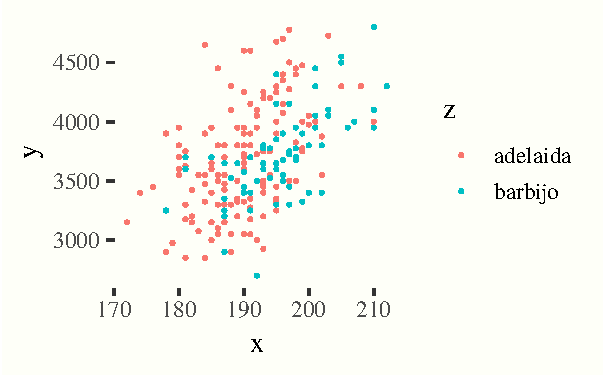
\includegraphics{TP-Labo-2_files/figure-latex/unnamed-chunk-10-1}
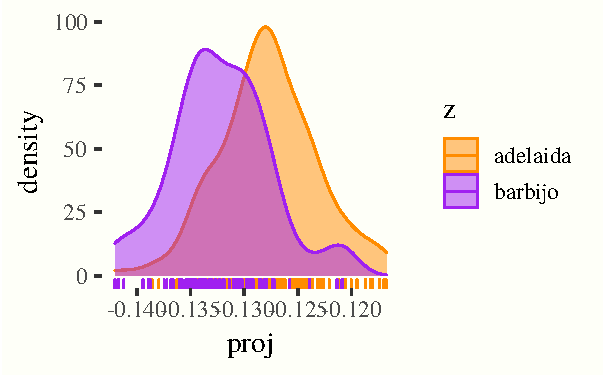
\includegraphics{TP-Labo-2_files/figure-latex/unnamed-chunk-10-2}

\hypertarget{referencias}{%
\section*{Referencias}\label{referencias}}
\addcontentsline{toc}{section}{Referencias}

\hypertarget{refs}{}
\leavevmode\hypertarget{ref-R-palmerpenguins}{}%
KB, Gorman, Williams TD, and Fraser WR. 2014. ``Ecological Sexual Dimorphism and Environmental Variability Within a Community of Antarctic Penguins (Genus Pygoscelis).'' \emph{PLoS ONE} 9(3) (e90081): --13. \url{https://doi.org/10.1371/journal.pone.0090081}.



\end{document}
